\documentclass[aspectratio=169]{beamer}
%\setbeameroption{show notes}

\usepackage{beamer_pre}


\title{Thesis meeting 2024/05/23}
\author{Albert R. S. Garde}
\date{\today}
	

\begin{document}

\frame{
	\maketitle
}

\begin{frame}[fragile=singleslide]
	\frametitle{Progress since last meeting}
    \begin{itemize}
        \item Looked into the literature.
        \item Investigated tasks for the models to solve.
        \item Attempted to get N2G working on \verb|gpt2-small| SAEs.
        \begin{itemize}
            \item Existing \verb|gpt2-small| SAEs have many features, which means that MAS data takes up a lot of space.
            \item I have ideas for solutions, but none are great.
        \end{itemize}
    \end{itemize}
\end{frame}
\begin{frame}[fragile=singleslide]
    \frametitle{Topics for meeting}
    \begin{itemize}
        \item Clarification of terms
        \item Plan for thesis content
    \end{itemize}
\end{frame}
\begin{frame}[fragile=singleslide]
    \frametitle{Clarification of terms}
    \begin{itemize}
        \item Language model: A generative model like the GPTs. 
        \begin{itemize}
            \item BERT is not an example of this type of model, since the attention is bidirectional.
        \end{itemize}
        \item N2G model: A model that models the \emph{activation pattern} of a single feature in a language model.
        It says nothing directly about the model behaviour as a whole, e.g. next token predictions.
        \item SAE: An autoencoder with a single hidden layer that is trained on the activations of a single layer of the model 
        in a way so that the hidden layer activations are more interpretable than the direct model activations.
    \end{itemize}
\end{frame}
\begin{frame}[fragile=singleslide]
    \frametitle{Plan for thesis content}
    \begin{itemize}
        \item First part: Literature review of SAEs specifically.
        This will include a short introduction to interpretability in general including the stuff covered by Bertology.
        \item Second part: Experiments with N2G on SAEs.
        I have 3 ideas for this. 
        For all of them comparing MLP neurons to SAE features is interesting.
        \begin{itemize}
            \item How does N2G performance on features compare with other interpretability methods and interpretability metrics?
            These include manual interpretability, automated interpretability, and sparsity.
            \item Find a task for the language model to solve. 
            Guess what N2G models of relevant features would look like.
            See if performance degrades when ablating(removing) these features.
            \item Investigate the universality hypothesis.
            Do features with the same N2G models appear across many different models?
            This would require us to formalize what we mean by "same N2G model".
        \end{itemize}
    \end{itemize}
\end{frame}
\begin{frame}[fragile=singleslide]
    \frametitle{Tasks}
    \begin{itemize}
        \item \verb|gelu-11| is far too underpowered for any task.
        \item The largest model we can comfortably work with is \verb|gpt2-small|, the largest we can practically work with is \verb|gpt2-xl|, and thats something of a stretch.
        These models are still underpowered for many interesting tasks.
        \item A possible task is correctly continuing the string \verb|The cat is sm| by completing a word.
        \item Basically all models can do this task, and I expected removing neurons activting on \verb|sm| to make the task harder, but this is not the case.
    \end{itemize}
    \begin{center}
        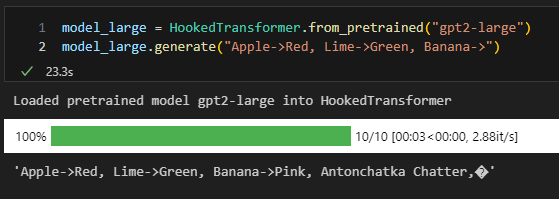
\includegraphics[scale=0.6]{images/fruit_colors.png}
    \end{center}
\end{frame}

\end{document}